\documentclass[11pt, a4paper]{report}

\usepackage[left=3.5cm,right=3.5cm,top=3cm,bottom=3.5cm]{geometry}
\usepackage{amsmath,amssymb,amsthm}
\usepackage{algorithm}
\usepackage{algpseudocode}
\usepackage{dsfont}
\usepackage{float}
\usepackage{graphicx}
\usepackage{hyperref}
\usepackage{pgfplots}
\usepackage{tikz}
\usepackage{titlesec}
\usepackage[utf8]{inputenc}

\pgfplotsset{compat=1.18}
\usetikzlibrary{calc}

% \titleformat{\chapter}[display]
%   {\normalfont\bfseries}{}{0pt}{\Huge\thechapter\quad}

\newtheoremstyle{mydefinition}
  {10pt} % space above the definition
  {10pt} % space below the definition
  {} % font of the body (empty means standard)
  {0pt} % no indentation
  {\bfseries} % font of the header
  {.} % punctuation after the header
  { } % space after the header
  {} % header specification (empty means standard)

\theoremstyle{mydefinition}
\newtheorem{definition}{Definition}
\newtheorem{theorem}{Theorem}
\newtheorem{lemma}{Lemma}

\newcommand{\1}{\mathds{1}}
\newcommand{\dt}{\;\mathrm{d}t}
\newcommand{\dx}{\;\mathrm{d}x}
\newcommand{\dphi}{\;\mathrm{d}\hat{\varphi}}
\newcommand{\C}{\mathbb{C}}
\newcommand{\E}{\mathbb{E}}
\newcommand{\K}{\mathbb{K}}
\newcommand{\N}{\mathbb{N}}
\newcommand{\R}{\mathbb{R}}
\newcommand{\SR}{\mathcal{S}(\R)}
\newcommand{\re}{\operatorname{Re}}
\newcommand{\im}{\operatorname{Im}}
\newcommand{\Cinfty}{\mathcal{C}^{\infty}}

\DeclareMathOperator\diag{diag}
\DeclareMathOperator\arcosh{arcosh}
\DeclareMathOperator\Tr{Tr}
\DeclareMathOperator\Real{Re}
\DeclareMathOperator\Imag{Im}

\begin{document}

\begin{titlepage}

    \newcommand{\HRule}{\rule{\linewidth}{0.5mm}} % Defines a new command for the horizontal lines, change thickness here
    
    \center
     
    %----------------------------------------------------------------------------------------
    %	HEADING SECTIONS
    %----------------------------------------------------------------------------------------
    
    \textsc{\LARGE University of Potsdam}\\[1.5cm] % Name of your university/college
    \textsc{\Large Bachelor Thesis}\\[0.5cm] % Major heading such as course name
    
    %----------------------------------------------------------------------------------------
    %	TITLE SECTION
    %----------------------------------------------------------------------------------------
    
    \HRule \\[0.4cm]
    { \huge \bfseries Investigation of Functionals of the Eigenvalues of Unitary Matrices}\\[0.4cm] % Title of your document
    \HRule \\[1.5cm]
     
    %----------------------------------------------------------------------------------------
    %	AUTHOR SECTION
    %----------------------------------------------------------------------------------------
    
    \begin{minipage}{0.4\textwidth}
    \begin{flushleft} \large
    \emph{Author:}\\
    Carina \textsc{Seidel} % Your name
    \end{flushleft}
    \end{minipage}
    ~
    \begin{minipage}{0.4\textwidth}
    \begin{flushright} \large
    \emph{Supervisor:} \\
    Dr. Thomas \textsc{Mach} % Supervisor's Name
    \end{flushright}
    \end{minipage}\\[2cm]
    
    % If you don't want a supervisor, uncomment the two lines below and remove the section above
    %\Large \emph{Author:}\\
    %John \textsc{Smith}\\[3cm] % Your name
    
    %----------------------------------------------------------------------------------------
    %	DATE SECTION
    %----------------------------------------------------------------------------------------
    
    {\large \today}\\[2cm] % Date, change the \today to a set date if you want to be precise
    
    %----------------------------------------------------------------------------------------
    %	LOGO SECTION
    %----------------------------------------------------------------------------------------
    
    
\includegraphics{./Graphics/Uni Potsdam.png}\\[0.9cm] % Include a department/university logo - this will require the graphicx package
     
    %----------------------------------------------------------------------------------------
    
    \vfill % Fill the rest of the page with whitespace
    
    \end{titlepage}

\begin{abstract}
The eigenvalues of large matrices are of interest for a large variety of use cases.
Their calculation however grows increasingly complex with increasing matrix sizes.
Therefore, we seek to simplify this process by approximating functionals over the spectrum of a matrix.
This thesis is focussed on the spectral density or Denisty of States (DoS) among those.
\end{abstract}

\tableofcontents

\chapter{Introduction}
We begin this thesis by examining unitary matrices and their fundamental properties.
Next, we introduce the Cayley transform to finally approach the concept of spectral density.
Upon this we will be well-equipped to proceed with the investigation afterwards.

\section{Unitary Matrices}

We first recall two definitions for important real matrices that we then extend to complex matrices.
The index $^T$ marks the transpose of a matrix.
As common in literature, $I_n$ denotes the identity matrix of size $n$.

\begin{definition}[Symmetric matrix]
    Let $A$ be a real, square matrix of size $n$.
    Then $A$ is called \emph{symmetric} if $A^T = A$.
\end{definition}

The following definition is for matrices with their transpose as their inverse.

\begin{definition}[Orthogonal matrix]
    Let $A$ be a real, square matrix of size $n$.
    Then $A$ is called \emph{orthogonal} if $A^T \cdot A = A \cdot A^T = I_n$.
\end{definition}


Now we define the complex equivalent of a real symmetric matrix.
Here, $A^*$ denotes the \emph{conjugate transpose} (also called adjoint) of $A$, that is,
the matrix obtained by taking the transpose and then complex conjugating all entries.

\begin{definition}[Hermitian matrix]
    Let $A$ be a complex square matrix of size $n$.
    Then $A$ is called \emph{Hermitian} if $A^* = A$.
\end{definition}

Throughout this thesis, $A$ will denote a complex, square matrix of size $n$, unless stated otherwise.
When referring to a Hermitian matrix, we will use the letter $H$.

We now examine the eigenvalues of Hermitian matrices.

Let $H = H^*$ and $H v = \lambda v$ for a complex vector $v \neq \mathbf{0}$ of size $n$ and a scalar $\lambda \in \C$.
Consider now the inner product $ v^* v$.
Remember that $(A \cdot B)^* = B^* \cdot A^*$ holds for a matrix product,
and obviously ${(A^*)^*} = A$ for all matrices and vectors.

\[
    \lambda v^* v = v^* \left( \lambda v \right)
    = v^* \left( H v \right)
    = \left(v^* H \right) v
    = \left( H^* v \right)^* v
    = \left( H v \right)^* v
    = (\lambda v)^* v
    = \overline{\lambda} v^* v
\]

Since we have that $v \neq \mathbf{0}$ it follows that $v^* v \neq \mathbf{0}$
and therefore $\lambda = \overline{\lambda}$, that is to say $\lambda$ is real.
This means that all eigenvalues of Hermitian matrices are real numbers.
It follows that all eigenvalues of symmetric matrices are also real numbers,
since they are a special case of Hermitian matrices.
Now we can define the complex equivalent of orthogonal matrices:

\begin{definition}[Unitary matrix]
    A matrix $A$ is called \emph{unitary} if $A^* \cdot A = A \cdot A^* = I_n$.
\end{definition}

We will oftentimes denote unitary matrices by using $U$ as a reference.
It is easy to see that orthogonal matrices are a special case of unitary matrices,
since $A^T = A^*$ for all real matrices.\\
Consider a unitary matrix $U$ and an eigenpair $(\lambda, v)$ of $U$.
The complex conjugate of the eigenvalue equation $U v = \lambda v$ is

\[
    v^* U^* = v^* \overline{\lambda} = \overline{\lambda} v^*
\]

We calculate

\[
    v^* v = v^* I_n v = v^* U^* U v = v^* \overline{\lambda} \lambda v = \overline{\lambda} \lambda v^* v = \left| \lambda \right|^2 v^* v
\]

Similarly to above, we can divide by $v^* v$ to obtain

\[
    1 = \left| \lambda \right|^2 \implies \left| \lambda \right| = 1
\]

meaning that all eigenvalues of unitary matrices have a length of $1$ and are thus situated on the unit circle.
As they are a special case of unitary matrices, the same goes for orthogonal matrices.
This property is crucial, as it enables the application of the Cayley transform,
introduced in the following section.

There is a special group of matrices that all the matrices we have defined so far belong to.

\begin{definition}[Normal matrix]
    A matrix $A$ is called \emph{normal} if it commutes with its conjugate transpose,
    that is to say $A^* A = A A^*$.
\end{definition}

It is straightforward to see that both Hermitian and unitary matrices are normal matrices
and that the notion includes real symmetric and orthogonal matrices as special cases.\\
The spectral theorem states that normal matrices can be diagonalized by a unitary matrix.
That means, for any normal matrix $A$, there exists a unitary matrix $U$ such that $A = U \Lambda U^*$,
where $\Lambda = \diag(\lambda_1, \ldots, \lambda_n)$ with $\lambda_1, \ldots, \lambda_n$ being the eigenvalues of $A$.
This is essential for applying a function to a matrix, which we will get to in the next section.

\section{Cayley Transform}

Before giving the central definition of this section,
we will first extend the concept of functions to normal matrices,
allowing us to map one matrix to another.

\begin{definition}[Matrix function on normal matrices]
    Let $A$ be a normal matrix and let $f: \C \to \C$ be a function that is defined on the spectrum of $A$,
    $\sigma(A) = \{\lambda_1, \ldots, \lambda_n\}$.
    Then the \emph{matrix function} $f(A)$ is defined as
    \[
    f(A) := U f(\Lambda) U^* = U \diag(f(\lambda_1), \ldots, f(\lambda_n)) U^*
    \]
    where $U$ is the matrix of eigenvectors of $A$ and $\Lambda = \diag(\lambda_1, \ldots, \lambda_n)$ is the diagonal matrix of eigenvalues.
\end{definition}

Now we can define the \emph{Cayley transform}, which is a specific matrix function, 
that establishes a correspondence between Hermitian and unitary matrices,
allowing spectral properties to be translated between these two important classes.

For a complex number $z \in \mathbb{C}$ with $z \neq -i$, the Cayley transform is defined as
\[
\varphi(z) = \frac{i - z}{i + z}.
\]

This function maps the real line to the unit circle in the complex plane.

\vspace{0.5cm}

\begin{figure}[ht]
    \centering
    \begin{tikzpicture}

        % The real line
        \begin{axis}[
            axis lines = middle,
            name = realline,
            height = 4cm, width = 4cm,
            major tick length = 2ex,
            scale only axis,
            xlabel={$\re$},
            xlabel style = {
                at={(1.075,0.435)},
                anchor=south
            },
            ylabel={$\im$},
            ylabel style = {
                at={(0.415,1.07)},
                anchor=west
            },
            xmin = -2.5, xmax = 2.5,
            xtick = {-2,-1,1,2},
            ymin = -1.5, ymax = 1.5,
            ytick = {-1,1},
            yticklabels={$-i$,$i$}
        ]

            % (-\inf, -1)
            \addplot[
                domain = -3:-1,
                color = orange,
                style = thick
            ]
            ({x},{0});

            % [-1, 1]
            \addplot[
                domain = -1:1,
                color = blue,
                style = thick
            ]
            ({x},{0});

            % (1, \inf)
            \addplot[
                domain = 1:2.4,
                color = red,
                style = thick
            ]
            ({x},{0});

        \end{axis}

        % Cayley Transform
        \begin{axis}[
            at={(realline.east)},
            xshift=2.5cm,
            anchor=west,
            axis lines = middle,
            name = cayleytransform,
            height = 4cm, width = 4cm,
            scale only axis,
            xlabel={$\re$},
            xlabel style = {
                at={(1.075,0.435)},
                anchor=south
            },
            ylabel={$\im$},
            ylabel style = {
                at={(0.415,1.07)},
                anchor=west
            },
            ticks=none,
            xmin = -1.5, xmax = 1.5,
            ymin = -1.5, ymax = 1.5
        ]
            
            % Unit circle
            \addplot[
                domain = 0 : 2*pi,
                samples = 100
            ]
            ({cos(deg(x))}, {sin(deg(x))});

            % Image of (-\inf, -1)
            \addplot[
                domain = -200 : -1,
                color = orange,
                style = thick,
                samples = 1150
            ]
            ({(1 - x*x)/(1 + x*x)}, {(2*x)/(1 + x*x)});

            % Image of [-1, 1]
            \addplot[
                domain = -1 : 1,
                color = blue,
                style = thick,
                samples = 100
            ]
            ({(1 - x*x)/(1 + x*x)}, {(2*x)/(1 + x*x)});

            % Image of (1, \inf)
            \addplot[
                domain = 1 : 200,
                color = red,
                style = thick,
                samples = 1150
            ]
            ({(1 - x*x)/(1 + x*x)}, {(2*x)/(1 + x*x)});

        \end{axis}

        \path[->,out=45,in=135] 
            ($(realline.east)+(-0.5cm,1cm)$) edge
            node[auto,above] {$\varphi(z)$}
            ($(cayleytransform.west)+(0.5cm,1cm)$);

    \end{tikzpicture}
\end{figure}

% The real and imaginary values for the plots are calculated as follows:
%
%
% i - x    (i - x) * (i - x)     -1 - 2ix + x*x     -1 + x*x         -2x        1 - x*x         2x
% ----- = ------------------- = ---------------- = ---------- + i ---------- = --------- + i ---------
% i + x    (i + x) * (i - x)        -1 - x*x        -1 - x*x       -1 - x*x     1 + x*x       1 + x*x

For matrices, the Cayley transform maps a Hermitian matrix $H$ (with $i + H$ invertible) to a unitary matrix $U$ via
\[
U = (i - H)(i + H)^{-1}.
\]
The condition of $i + H$ being invertible is the same as requiring that $H$ does not have $-i$ as an eigenvalue.
If (and only if) that were the case, then we had $H v = -i v$ for some eigenvector $v \neq \mathbf{0}$,
and therefore 
\[
(i + H) v = i v + H v = i v + (-i v) = 0.
\]

Since Hermitian matrices have only real eigenvalues as discussed above, $-i$ can never be an eigenvalue.
Conversely, given a unitary matrix $U$ (with $U \neq -I_n$),
the inverse Cayley transform yields a Hermitian matrix:
\[
H = i (I_n - U)(I_n + U)^{-1}.
\]

This will be relevant later, as we can then use $\varphi$ to transform unitary matrices into symmetric ones and vice versa.

\subsection*{On the Choice of Random Unitary Matrices}


When generating random unitary matrices for numerical experiments,
it is important to ensure that their eigenvalues are distributed uniformly on the unit circle,
as predicted by random matrix theory.
A common approach is to generate a random complex matrix $A$ with independent standard normal entries
and then construct a unitary matrix from $A$ using either the QR decomposition or the singular value decomposition (SVD).
In the QR approach, $A$ is factored as $A = QR$, where $Q$ is unitary and $R$ is upper triangular.
The matrix $Q$ is then used as the random unitary matrix.
In the SVD approach, $A$ is factored as $A = U \Sigma V^*$,
and either $U$ or $V$ (both unitary) can be used as a random unitary matrix.
Although both methods produce unitary matrices, their statistical properties differ.
The SVD-based approach yields unitary matrices whose eigenvalues are uniformly distributed on the unit circle,
matching the theoretical prediction for random unitary matrices (the so-called Haar measure).
In contrast, the QR-based approach does not generally produce a uniform distribution of eigenvalues on the unit circle.
This distinction is important for applications where the spectral properties of random unitary matrices play a central role,
such as in the study of spectral densities.
For such purposes, the SVD-based construction is preferable,
as it ensures the correct statistical behavior of the eigenvalues.

\begin{figure}[htb]
    \centering
    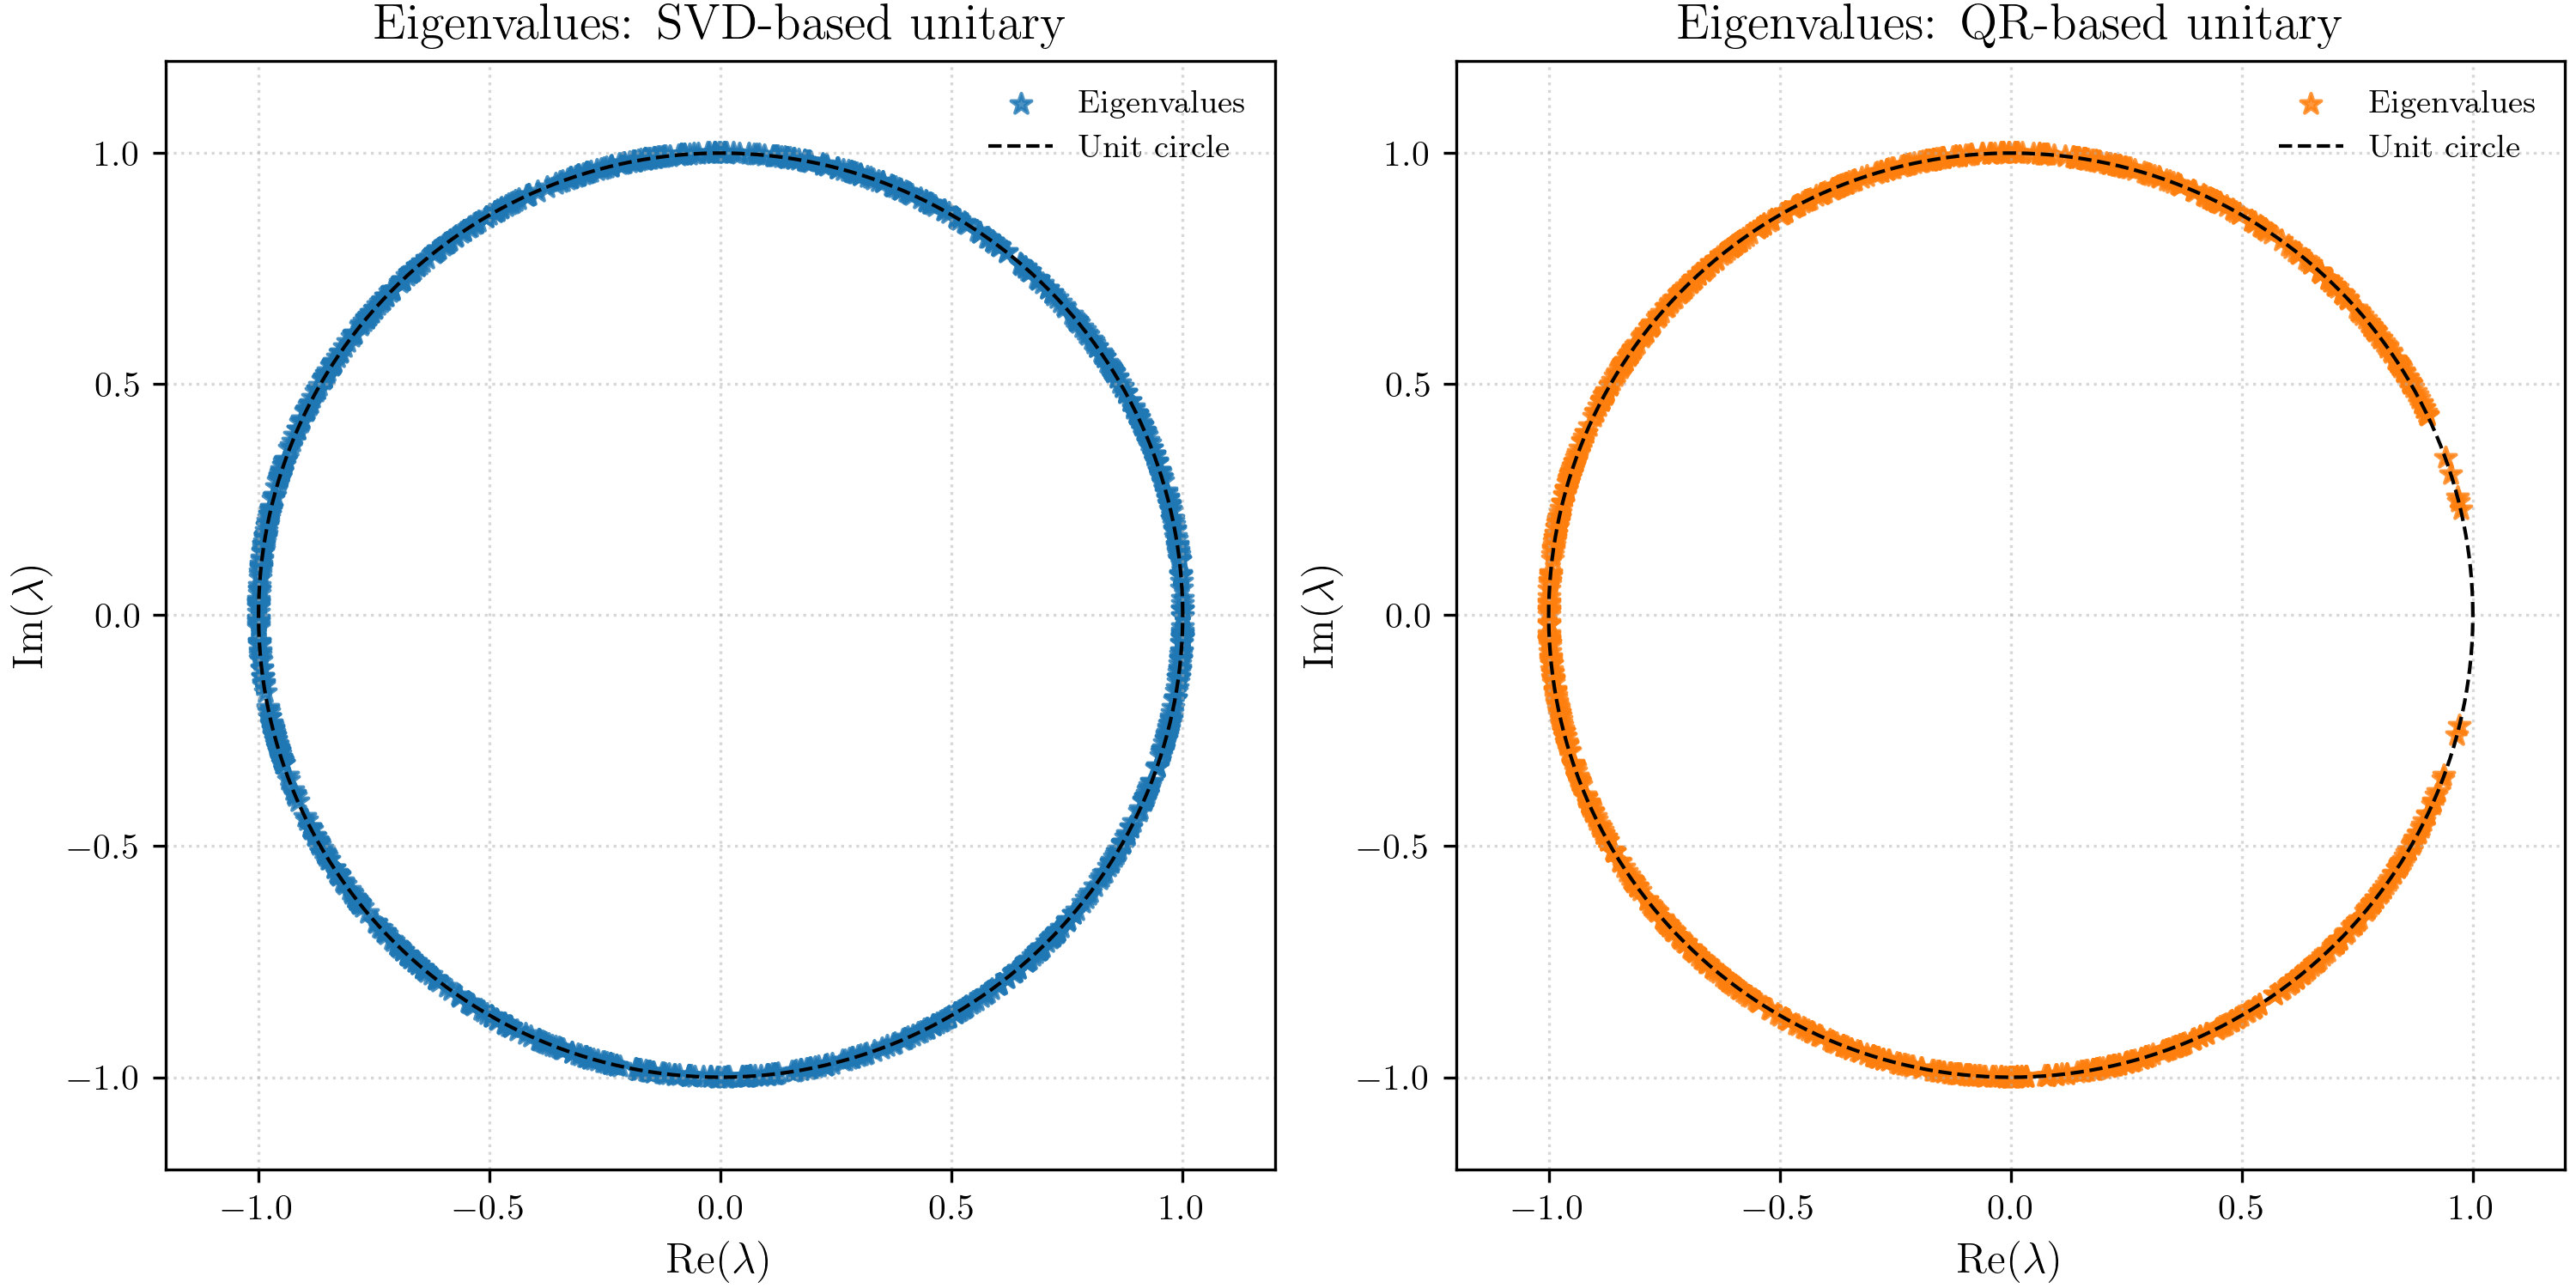
\includegraphics[width=1\textwidth]{Graphics/eigenvalue_comparison.png}
    \caption{Eigenvalue distributions of random unitary matrices generated via SVD and QR.}
    \label{fig:eigenvalue-comparison}
\end{figure}

\section{Spectral Density}

To get to the notion of the spectral density,
we will first need some more basic definitions to build on.
The reader is assumed to be familiar with the concepts of distributions.
Let us also recap that for $\Omega \subset \C^n$ open and non-empty,
a \emph{test function} is a smooth function with compact support defined on $\Omega$.
The space of all test functions on $\Omega$ is usually denoted by $\mathcal{E}$.

We will now look at an important case of a distribution

\begin{definition}[Dirac delta distribution]
    Let $\mathcal{E} = \Cinfty(\Omega)$ with $0 \in \Omega \subset \R^n$.
    Then
    $$\delta: \mathcal{E} \to \R, \quad f \mapsto f(0) \quad \text{with} \quad \delta(f) = \langle \delta, f \rangle = f(0)$$
\end{definition}

this distribution is often mistakenly referred to as a function,
although it is not a function in the classical sense.\\
The Dirac delta is characterized by the following property:

\[
\int\limits_{-\infty}^{\infty} f(x) \delta(x-a) \dx = \int\limits_{-\infty}^{\infty} f(x) \delta(a-x) \dx = f(a) \implies \int\limits_{-\infty}^{\infty} \delta(x-a) \dx = 1.
\]

This means that the Dirac delta distribution is zero everywhere except at the point $a$,
where it is infinitely high, such that the integral over it equals $1$.
We now have all the tools we need to define the central concept of this thesis:

\begin{definition}[Spectral density]
    Let $H$ be hermitian and sparse.
    For $x \in \R$, the \emph{spectral density} is then defined as
    \[
    \phi(x) = \frac{1}{n} \sum_{j=1}^{n} \delta(x - \lambda_j)
    \]
    where $\delta$ is the Dirac delta distribution
    and $\lambda_j$ are the eigenvalues of $H$ in non-descending order.
\end{definition}

The number of eigenvalues in an interval $[a, b]$ can then be counted in the following manner:

\begin{equation} \label{eq:nu_a_b}
    \nu_{[a, b]} = \int\limits_a^b \sum_j \delta(t - \lambda_j) \dt \equiv \int\limits_a^b n \phi(t) \dt
\end{equation}

Random matrix theory tells us that the eigenvalues of random unitary matrices are distributed uniformly on the unit circle.
Thus, we would expect the spectral density to be uniformly distributed on the unit circle as well.
This is important as we think of the choice of random unitary matrices.

If we generate a random complex square matrix $A$,
there are multiple ways to obtain a unitary matrix $U$.
We will now compare the svd with the qr decomposition.

Before we can proceed to the motice of this thesis, we will need to define the following space:

\begin{definition}[Schwartz space over $\R$] \label{def:Schwartz space}
    The \emph{Schwartz space} over $\R$ consists of all smooth functions $f$ that decay rapidly to zero as $|x|$ approaches infinity \cite{richtmyer}.
    Formally,
    \[
    \SR := \left\{f \in \Cinfty(\R) \mid \forall p, k \in \N_0: \sup_{x \in \R} \left| x^p f^{(k)}(x) \right| < \infty \right\}
    \]
\end{definition}

\chapter{Regularization of the Spectral Density}
Because of its ability to capture the distribution of eigenvalues, the spectral density of a matrix is a crucial concept in various fields. For example, in quantum mechanics, it describes the density of energy states~\cite{reichl,sakurainapolitano}; in signal processing, it describes how power is distributed over frequency~\cite{oppenheimschafer, mitra}; and in vibration analysis, it characterizes how energy is distributed among the natural frequencies of a structure~\cite{nortonkarczub}. However, two main challenges arise when defining and computing the spectral density for a matrix~$H$.

Firstly, the eigenvalues of~$H$ are typically not known in advance. If they were, computing the spectral density would be straightforward, but this is rarely the case for large matrices. Secondly, the spectral density is defined using the Dirac delta distribution, which is not a conventional function and cannot be evaluated pointwise. This makes direct computation infeasible, especially for large matrices where eigenvalue decomposition is prohibitively expensive.

\section{Regularization and Polynomial Expansion}
To address the second challenge, a fundamental idea is to replace the delta distribution by a regular function~$f$ with similar properties. To be effective, the regularizing function should be normalized, meaning it satisfies the condition
\[
    \int\limits_{\mathbb{R}} f(x)\, dx = 1;
\]
localized, meaning it is significant only near the origin; and sufficiently smooth to avoid introducing artificial oscillations or numerical instability. Sufficiently smooth is to say that the regularizing function should have continuous derivatives up to at least a certain order. Making sure~$f$ decays rapidly away from zero ensures that the regularized spectral density reflects the true distribution of eigenvalues without excessive broadening.

The choice of regularizing function~$f$ is crucial for both the accuracy and stability of spectral density approximations. While a single regular function~$f$ to replace the Dirac delta distribution might be hard to find, a powerful approach is to expand the spectral density in terms of a basis of functions such as $f_1, f_2, \ldots$ satisfying the above mentioned requirements to allow for greater flexibility and accuracy. A perfect approximation would satisfy equality in the sense of distributions, meaning that it holds when integrated against a test function~$g \in \SR$, the Schwartz space of rapidly decreasing functions from Definition ~\ref{def:Schwartz_space}. More precisely, this can be expressed as
\[
\int\limits_{-\infty}^{\infty} \phi(x) g(x) \dx = \int\limits_{-\infty}^{\infty} \sum_{k=0}^{\infty} \mu_k f_k(x) g(x) \dx.
\]
If this equation holds true for all test functions~$g$, it can be simplified to

\begin{equation} \label{eq:polynomial_expansion}
    \phi(x) = \sum_{k=0}^{\infty} \mu_k f_k(x),
\end{equation}
which we call our \emph{polynomial expansion}. Now we need to determine the coefficients~$\mu_k$ in the expansion. The easiest way to do this is to isolate a single coefficient~$\mu_k$, as we will do in this following section.

\section{Orthogonal Polynomial Expansions and Basis Selection}
For a given interval~$[a, b]$, we consider a non-negative weight function $w: [a, b] \to \R$. The inner product for two functions $f, g: [a, b] \to \R$ is then defined as
\begin{equation} \label{eq:inner_product}
    \left \langle f, g \right \rangle_w := \int\limits_a^b w(x) f(x) g(x) \dx.
\end{equation}
Now define~$\hat{\phi}_w$ as the product of spectral density with the inverse of one such weight function $w$:
\begin{equation} \label{eq:phi_hat}
\hat{\phi}_w(x) := w^{-1}(x) \, \phi(x) =  w^{-1}(x) \; \frac{1}{n} \sum_{j = 1}^n \delta(x - \lambda_j)
\end{equation}
Similarly to \eqref{eq:polynomial_expansion}, we can then express the modified spectral density~$\hat{\phi}_w$ as an infinite series of regular functions~$f_k$:
\begin{equation} \label{eq:phi_hat_polynomial_expansion}
    \hat{\phi}_w(x) = \sum_{k = 0}^{\infty} \mu_k f_k(x)
\end{equation}
To isolate a single coefficient $\mu_k$, it is useful that the basis functions $f_k$ are \emph{orthogonal} with respect to some weight function $w(x)$. This means that for any two indices $k$ and $l$, we have:
\[
\left \langle f_k, f_l \right \rangle_w = \int \limits_{a}^b w(x) f_k(x) f_l(x) \dx = 0 \quad \text{for } k \neq l.
\]
It is also advantageous to use an orthogonal polynomial base which satisfies an explicitly known three-term recurrence relation of the form
\[
f_{k}(x) = (A_k x + B_k) f_{k-1}(x) + C_k f_{k-2}(x),
\]
where $A_k, B_k, C_k \in \R$ are coefficients that may depend on~$k$ and the weight function. This three-term recurrence relation would allow us to efficiently compute the polynomials by using only vector instead of matrix multiplications. This entails the polynomials being degree-graded, that is to say $\deg(f_k) = k$ for each~$k$.

It follows from Favard's theorem~\cite[Thm.~2.1]{szego1975} that for every possible choice of weight function $w$ and interval $[a, b]$, there exists a orthogonal polynomial basis $\{f_k\}_{k=0}^{\infty}$ that is unique up to normalization and satisfies the above properties. Since there are infinitely many choices for the weight function, we have infinitely many choices for the basis functions, and we can choose one that is convenient for our purposes. Some well-studied examples of orthogonal polynomial bases are the Chebyshev polynomials, Legendre polynomials, and Hermite polynomials. These are widely used in numerical analysis and approximation theory due to their favorable convergence properties and computational efficiency~\cite{masonhandscomb}. We focus on Chebyshev polynomials in the next chapter.

Finally, to ensure that our chosen regularizing functions provide meaningful and accurate approximations of the spectral density in practice, we turn to practical strategies for validation and computation. These considerations are the focus of the next section.

\section{Efficient Numerical Methods}
For real symmetric matrices, a variety of efficient methods have been developed to approximate the spectral density, often relying on this regularization principle~\cite{weisse2006,linsaadyang14,golub2013matrix}. However, many problems in mathematics and physics naturally lead to complex Hermitian or even unitary matrices, for which the spectral density is less straightforward to compute. In this thesis, we generalize the established approaches for Chebyshev polynomials from the real symmetric case to the Hermitian case, and further broaden the scope to unitary matrices. This is achieved by first applying the Cayley transform, which provides a bridge between Hermitian and unitary matrices and allows us to transfer techniques and insights between these classes.

One intuitive approach by~\cite{linsaadyang14} is to select an interval~$I \subset \R$ containing the spectrum of~$H$, and divide it into~$k$ subintervals using points~$\{t_i\}_{i=1}^k$. By applying Sylvester's law of inertia~\cite{sylvester1852}, we can count the number of eigenvalues in each subinterval, resulting in a histogram. Then we could approximate the average value of~$\phi(x)$ in that interval using the fact that the number of eigenvalues in the interval can formally be expressed as
\begin{equation} \label{eq:nu_a_b}
    \nu_{[t_i, t_{i+1}]} := \int\limits_{t_i}^{t_{i+1}} \sum_j \delta(t - \lambda_j) \dt \equiv \int\limits_{t_i}^{t_{i+1}} n \phi(t) \dt.
\end{equation}
This provides useful reference points for assessing the shape of the regularized spectral density and evaluating whether the chosen functions~$f_k$ yield an appropriate approximation.

Using Sylvester's law of inertia requires computing a decomposition of~$A - t_i I = LDL^T$ for all~$t_i$~\cite{golub2013matrix}. While this is efficient for certain structured matrices~\cite{bennermach2012}, it becomes computationally expensive or impractical for large, unstructured matrices.

This motivates the development and use of efficient numerical methods that can approximate the spectral density using only matrix-vector multiplications, which scale better with matrix size. In this thesis, we explore one such method, the so-called Kernel polynomial method or KPM for short, which makes the computation of spectral densities feasible for large-scale problems. These advances have the potential to impact a wide range of scientific and engineering disciplines where understanding the spectral properties of large matrices is crucial.

\chapter{Kernel Polynomial Method}
\section{Overview}
There exists a whole class of methods, all of which called the kernel polynomial method, or KPM for short.
They are powerful tools for approximating the spectral density of matrices.
We will focus on the main approach in the following.\\
As the name suggests, the KPM is a polynomial extension of the spectral density.
The coefficients of the polynomials are derived from the method of moments,
in order to obtain an estimator function as in statistics.

The method is based on a corollary of the following generalized theorem:

\begin{theorem}
    Let $A \in \C^{n \times n}$ be a normal matrix with spectral decomposition
    \[
    A = U \Lambda U^* \quad \text{where} \quad UU^* = I_n \text{ and } \Lambda = \diag(\lambda_1, ..., \lambda_n)
    \]
    Let $\beta, v \in \C^n$ with $v = U\beta$.
    Suppose $v$ is a random vector whose entries $v_i$ are independent and identically distributed standard complex normal variables,
    i.e., $v_i \sim_\text{i.i.d.} \mathcal{N}_\C(0, 1)$, meaning $\Real(v_i), \Imag(v_i)$ are independent $\mathcal{N}(0, \frac{1}{2})$.
    Then
    \begin{equation} \label{eq:complex_normal_vector}
        \E[v] = 0 \quad \text{and} \quad \E[v v^*] = I_n,
    \end{equation}
    and it follows that
    \[
    \E[\beta] = 0 \quad \text{and} \quad \E[\beta \beta^*] = I_n.
    \]
\end{theorem}


\begin{proof}[Proof of Theorem 1]
    Since the expectation operator is linear, it holds that
    \[
    \E[v] = \E[U\beta] = U\E[\beta] = 0 \implies \E[\beta] = 0
    \]
    Furthermore it holds that
    \[
    I_n = \E[vv^*] = \E[(U\beta)(U\beta)^*] = \E[U\beta \beta^*U^*] = U \E[\beta \beta^*]U^*
    \]
    Multiplying both sides with $U^*$ and $U$ yields:
    \[
    U^* I_n U = U^* U \E[\beta \beta^*]U^* U = \E[\beta \beta^*]
    \]
    Since $U$ is unitary, we have shown that $\E[\beta \beta^*] = I_n$.
\end{proof}


\vspace{0.5 cm}
This theorem has a nice corollary when investigating a matrix function $f(A)$.
In that case, we have

\begin{align*}
    \E\left[v^* f(A) v\right] &= \E\left[(U\beta)^* f(U\Lambda U^*) (U\beta)\right] \\
        &= \E\left[\beta^* U^* U f(\Lambda) U^* U \beta\right] \\
        &= \E\left[\beta^* f(\Lambda) \beta\right] \\
        &= \E\left[\sum_{j = 1}^n |\beta_j|^2 f(\lambda_j) \right] \\
        &= \sum_{j = 1}^n f(\lambda_j) \E\left[ |\beta_j|^2 \right] \\
        &= \sum_{j = 1}^n f(\lambda_j)
\end{align*}

or, more concisely,
\begin{equation} \label{eq:theorem_result}
    \E\left[v^* f(A) v\right] = \Tr(f(A)).
\end{equation}

\section{Polynomial Extension with Chebyshev polynomials}
We assume Chebyshev polynomials to be a good fit for the polynomial extension of the Dirac delta distribution
because of the many great properties we will see now. First, let's look how Chebyshev polynomials are defined.
Using the trigonometric functions, they can be expressed as follows:

\[ T_k(x) =
\begin{cases}

\cos(k \arccos(x))                & \quad \text{for } k \in [-1, 1]\\
    \cosh(k \arcosh(x))           & \quad \text{for } k > 1\\
    (-1)^k \cosh(k \arcosh(-x))   & \quad \text{for } k < -1
\end{cases}
\]

We will only use the formula $T_k(x) = \cos(k \arccos(x))$.
This means to only consider matrices, which have eigenvalues within the intervall $[-1, 1]$.
In the case that this condition should not be fulfilled, the eigenvalues can be transformed accordingly.
For this, let $\lambda_{lb}$ and $\lambda_{ub}$ be the lower and upper bound for the eigenvalues of $A$, respectively.
To find these, well-established methods like the Gershgorin circle theorem can be used.

Define
\[
c := \frac{\lambda_{lb} + \lambda_{ub}}{2} \quad \text{and} \quad d := \frac{\lambda_{ub} - \lambda_{lb}}{2}
\]
Then, the matrix $B = \frac{A - c*I_n}{d}$ has eigenvalues in the interval $[-1, 1]$.
A visualization of this is linked in the appendix.


Another way to define Chebyshev polynomials is by calculating them using the recursion formula
\[
T_{k + 1}(x) = 2xT_k(x) - T_{k - 1}(x),
\]
where the starting conditions are given by $T_0(x) = 1$ and $T_1(x) = x$.

Additionally, note that the result in equation \ref{eq:theorem_result} says, that

\begin{equation} \label{eq:Chebyshev_trace}
    \E\left[\,v^T T_k(A) v\,\right] = \Tr\left(T_k(A)\right).
\end{equation}

This result will be central in the following discussion.


Now, let
\begin{equation} \label{eq:weight_function}
    h(x) = \frac{1}{\sqrt{1 - x^2}}
\end{equation}
be a weight function.
Another property of Chebyshev polynomials is
that they are \emph{orthogonal} in terms of the scalar product weighted with $h$:

\[
\left \langle f, g \right \rangle = \int_{-1}^1 \frac{1}{\sqrt{1 - x^2}} \cdot f(x) \cdot g(x) \dx.
\]

This means that

\[
\int_{-1}^1 \frac{1}{\sqrt{1 - t^2}} \cdot T_k(t) \cdot T_l(t) \dt =
\begin{cases}
    0               & \quad \text{for } k \neq l\\
    \pi             & \quad \text{for } k = l = 0\\
    \frac{\pi}{2}   & \quad \text{for } k = l \neq 0
\end{cases}
\]

\section{Approximating the spectral density}
Now multiply the spectral density with the inverse of the weight function \ref{eq:weight_function}:
\[
\hat{\phi}(x) = \sqrt{1 - x^2} \phi(x) = \sqrt{1 - x^2} \, \cdot \, \frac{1}{n} \sum_{j = 1}^n \delta(x - \lambda_j)
\]
Let $g \in \SR$, the Schwartz space defined in definition \ref{def:Schwartz space},
and $\mu_k \in \R$ coefficients to be determined such that the following equation holds:

\begin{equation} \label{eq:distribution_equality}
    \int \limits_{-1}^1 \hat{\phi}(t) g(t) \dt = \int \limits_{-1}^1 \sum_{k = 0}^{\infty} \mu_k T_k(t) g(t) \dt
\end{equation}

If this is true for arbitrary $g \in \SR$, we can simplify our equation \ref{eq:distribution_equality} to

\begin{equation} \label{eq:Chebyshev-Expansion}
    \hat{\phi}(x) = \sum_{k = 0}^{\infty} \mu_k T_k(x)
\end{equation}


Now utilize the orthogonality of the Chebyshev polynomials, to calculate a specific coefficient $\mu_k$:

\begin{align*}
    & \; \; \sum_{l = 0}^{\infty} \mu_l T_l(t) = \hat{\phi}(t) \\
    \implies & \left(\sum_{l = 0}^{\infty} \mu_l T_l(t)\right) \cdot T_k(t) = \hat{\phi}(t) \cdot T_k(t)\\
    \implies & \int_{-1}^1 \frac{1}{\sqrt{1 - t^2}} \cdot \left(\sum_{l = 0}^{\infty} \mu_l T_l(t)\right) \cdot T_k(t) \dt = \int_{-1}^1 \frac{1}{\sqrt{1 - t^2}} \cdot \hat{\phi}(t) \cdot T_k(t) \dt\\
    \implies & \mu_k \cdot \frac{\pi}{2 - \delta_{k0}} = \int_{-1}^1 \frac{1}{\sqrt{1 - t^2}} \cdot \sqrt{1 - t^2} \cdot \phi(t) \cdot T_k(t) \dt\\
    \implies & \mu_k = \frac{2 - \delta_{k0}}{\pi} \cdot \int_{-1}^1 \phi(t) \cdot T_k(t) \dt\\
\end{align*}

By applying the Dirac delta distribution we obtain:
\begin{align*}
    \mu_k = \frac{2 - \delta_{k0}}{\pi} \cdot \int_{-1}^1 \phi(t) \cdot T_k(t) \dt &= \frac{2 - \delta_{k0}}{\pi} \cdot \int_{-1}^1 \frac{1}{n} \sum_{j = 1}^n \delta(t - \lambda_j) \cdot T_k(t) \dt \\
    &= \frac{2 - \delta_{k0}}{n \pi} \sum_{j = 1}^n T_k(\lambda_j)\\
    &= \frac{2 - \delta_{k0}}{n \pi} \Tr(T_k(A))
\end{align*}

Now let $n_{\text{vec}} \in \R$ and consider vectors $v_0^{(1)}, v_0^{(2)}, \dots, v_0^{(n_{\text{vec}})}$,
which are chosen randomly from the standard normal distribution,
that is to say $\E[v_0^{(k)}] = 0$ und $\E\left[v_0^{(k)}\left(v_0^{(k)}\right)^T\right] = I_n$.
It follows from equation \ref{eq:Chebyshev_trace} that
\[
\zeta_k = \frac{1}{n_{\text{vec}}} \sum_{l = 1}^{n_{\text{vec}}} \left( v_0^{(l)} \right)^T T_k(A) v_0^{(l)}
\]
is a good estimator for $\Tr(T_k(A))$ and therefore
\[
\mu_k \approx \frac{2 - \delta_{k0}}{n \pi} \zeta_k
\]

In order to determine the $\zeta_k$, let $v_0 \equiv v_0^{(l)}$
Using the recursion formula for Tschebyschev polynomials, we can calculate
\[
T_{k + 1}(A)v_0 = 2 A T_k(A) v_0 - T_{k - 1}(A) v_0
\]
For $v_k \equiv T_k(A)v_0$ it also holds that
\[
v_{k + 1} = 2 A v_k - v_{k - 1}
\]

With this we are fully equpped for the final calculation and the goal of the KPM is reached:
Instead of having to multiply matrices with other matrices, it now suffices to multiply matrices with vectors.
Now we can approximate $\phi(x)$ as closely as we like.
As aforementioned, it is not always desirable to have an infinitely exact approximation.
Since it holds that
\[
\lim \limits_{k \to \infty} \mu_k \to 0
\]
and we are only interested in $T_k(x)$ with $k \leq M$\\
Therefore we estimate $\phi$ with
\begin{equation} \label{eq:Angenäherte Spektraldichte}
    \tilde{\phi}_M(x) = \frac{1}{\sqrt{1 - x^2}} \sum_{k = 0}^{M} \mu_k T_k(x)
\end{equation}

The following pseudo code is based on \cite[p.~10]{linsaadyang14} and summarizes the steps described above.
The implementation is done in Python, and linked in the appendix.

\begin{algorithm}
    \caption{The Kernel Polynomial Method}\label{alg:cap}
    \begin{algorithmic}[5]
    \Require $A = A^* \in \mathbb{C}^{n \times n}$ with eigenvalues in the intervall $[-1, 1]$
    \Ensure Estimated spectral density \{$\tilde{\phi}_M(t_i)$\}\\
    \For{$k = 0 : M$}
    \State $\zeta_k \gets 0$
    \EndFor
    \For{$l = 1 : n_{\text{vec}}$}
    \State $\text{Choose a random new vector } v_0^{(l)}\text{;}$ \Comment{$v_{0_i}^{(l)} \sim_\text{ i.i.d. } \mathcal{N}(0, 1)$}
    \For{$k = 0 : M$}
    \State $\text{Calculate } \zeta_k \gets \zeta_k + \left( v_0^{(l)} \right)^T v_k{(l)}\text{;}$  
    \If{$k = 0$}
    \State $v_1^{(l)} \gets A v_0^{(l)}$
    \Else
    \State $v_{k+1}^{(l)} \gets 2 A v_k^{(l)} - v_{k-1}^{(l)}$ \Comment{Three term recursion}
    \EndIf
    \EndFor
    \EndFor
    \For{$k = 0 : M$}
    \State $\zeta_k \gets \frac{\zeta_k}{n_{\text{vec}}}$
    \State $\mu_k \gets \frac{2 - \delta_{k0}}{n \pi} \zeta_k$
    \EndFor
    \State $\text{Evaluate } \tilde{\phi}_M(t_i) \text{ with equation } \ref{eq:Angenäherte Spektraldichte}$
    \end{algorithmic}
\end{algorithm}

Applying the Cayley transform to an arbitrary unitary matrix $U$ yields a Hermitian matrix $H$;
and as this is the case, the KPM can be applied to unitary matrices as well.

\chapter{Results}
We now want to use the algorithm from the previous section to compute the spectral density of a unitary matrix~$U$. In order to assess the results, we need to compare the computed spectral density with the theoretical one. The problem is that the spectral density we defined applies to the real line, while the eigenvalues of a unitary matrix lie on the unit circle in the complex plane. To overcome this, we need to transform it a little first.

\section{Transformation of the Spectral Density for Comparison}

The exact spectral density at a point $x$ on the real line is given by
\[
\phi(x) = \sum_{i=1}^n \delta(x - \lambda_i),
\]
where $\delta$ is the Dirac delta function. For a regularized, smoothed delta function, one simply evaluates the regularization function at $x - \lambda_i$ for all $i$ and sums the result. We use Gaussian regularization in our implementation, with the Gaussian function defined as
\[
    g_\sigma(x) = \frac{1}{\sqrt{2\pi} \sigma} e^{-\frac{x^2}{2\sigma^2}},
\]
where $\sigma$ is the standard deviation of the Gaussian. This $\sigma$ is often called the \emph{target resolution} \cite{linsaadyang14}; the smaller it is, the higher the resolution of the spectral density. We need to balance high resolution for exactness with easier approximation for larger $\sigma$.
Then we replace the Dirac delta function in the spectral density with the Gaussian regularization function:
\[
    \phi_\sigma(x) := \sum_{i=1}^n g_\sigma(x - \lambda_i).
\]


However, we defined the spectral density only on the real line, while the eigenvalues of a unitary matrix lie on the unit circle. To be able to evaluate $\phi_\sigma(z)$ for $z \in \C$, we use the inverse Cayley transform $\varphi^{-1}(z) = i\frac{1 - z}{1 + z}$, which maps $z \in \mathbb{S}^1$ to $x \in \R$, and evaluate $\phi_\sigma(\varphi^{-1}(z))$. According to the standard change-of-variables formula for probability densities, this requires multiplying by the Jacobian determinant to ensure correct normalization:
\[
    \hat{\phi}_\sigma(z) = \phi_\sigma(\varphi^{-1}(z)) \, \frac{(\varphi^{-1}(z))^2 + 1}{2} = \sum_{i=1}^n g_\sigma(\varphi^{-1}(z) - \lambda_i) \, \frac{(\varphi^{-1}(z))^2 + 1}{2}.
\]
An exact computation for the Jacobian determinant is found in the appendix.

Before we can plot the spectral density of a unitary matrix $U$ on the unit circle, we need to consider which random unitary matrices to use for our numerical experiments. The choice of random unitary matrices is crucial, as it affects the distribution of eigenvalues and thus the spectral density we want to compute.

\section{The Choice of Random Unitary Matrices}

When generating random unitary matrices for numerical experiments, it is important to ensure that their eigenvalues are distributed uniformly on the unit circle, as predicted by random matrix theory~\cite{mezzadri2007}. A common approach is to generate a random complex matrix $A$ with independent standard normal entries and then construct a unitary matrix from $A$ using either the QR decomposition or the singular value decomposition (SVD). In the QR approach, $A$ is factored as $A = QR$, where $Q$ is unitary and $R$ is upper triangular. The matrix $Q$ is then used as the random unitary matrix. In the SVD approach, $A$ is factored as $A = U \Sigma V^*$, and either $U$ or $V$ (both unitary) can be used as a random unitary matrix.
Although both methods produce unitary matrices, their statistical properties differ.
The SVD-based approach yields unitary matrices whose eigenvalues are uniformly distributed on the unit circle,
matching the theoretical prediction for random unitary matrices (the so-called Haar measure)~\cite{mezzadri2007}.
In contrast, the QR-based approach does not generally produce a uniform distribution of eigenvalues on the unit circle. This distinction is important for applications where the spectral properties of random unitary matrices play a central role, such as in the study of spectral densities.

\begin{figure}[H]
    \centering
    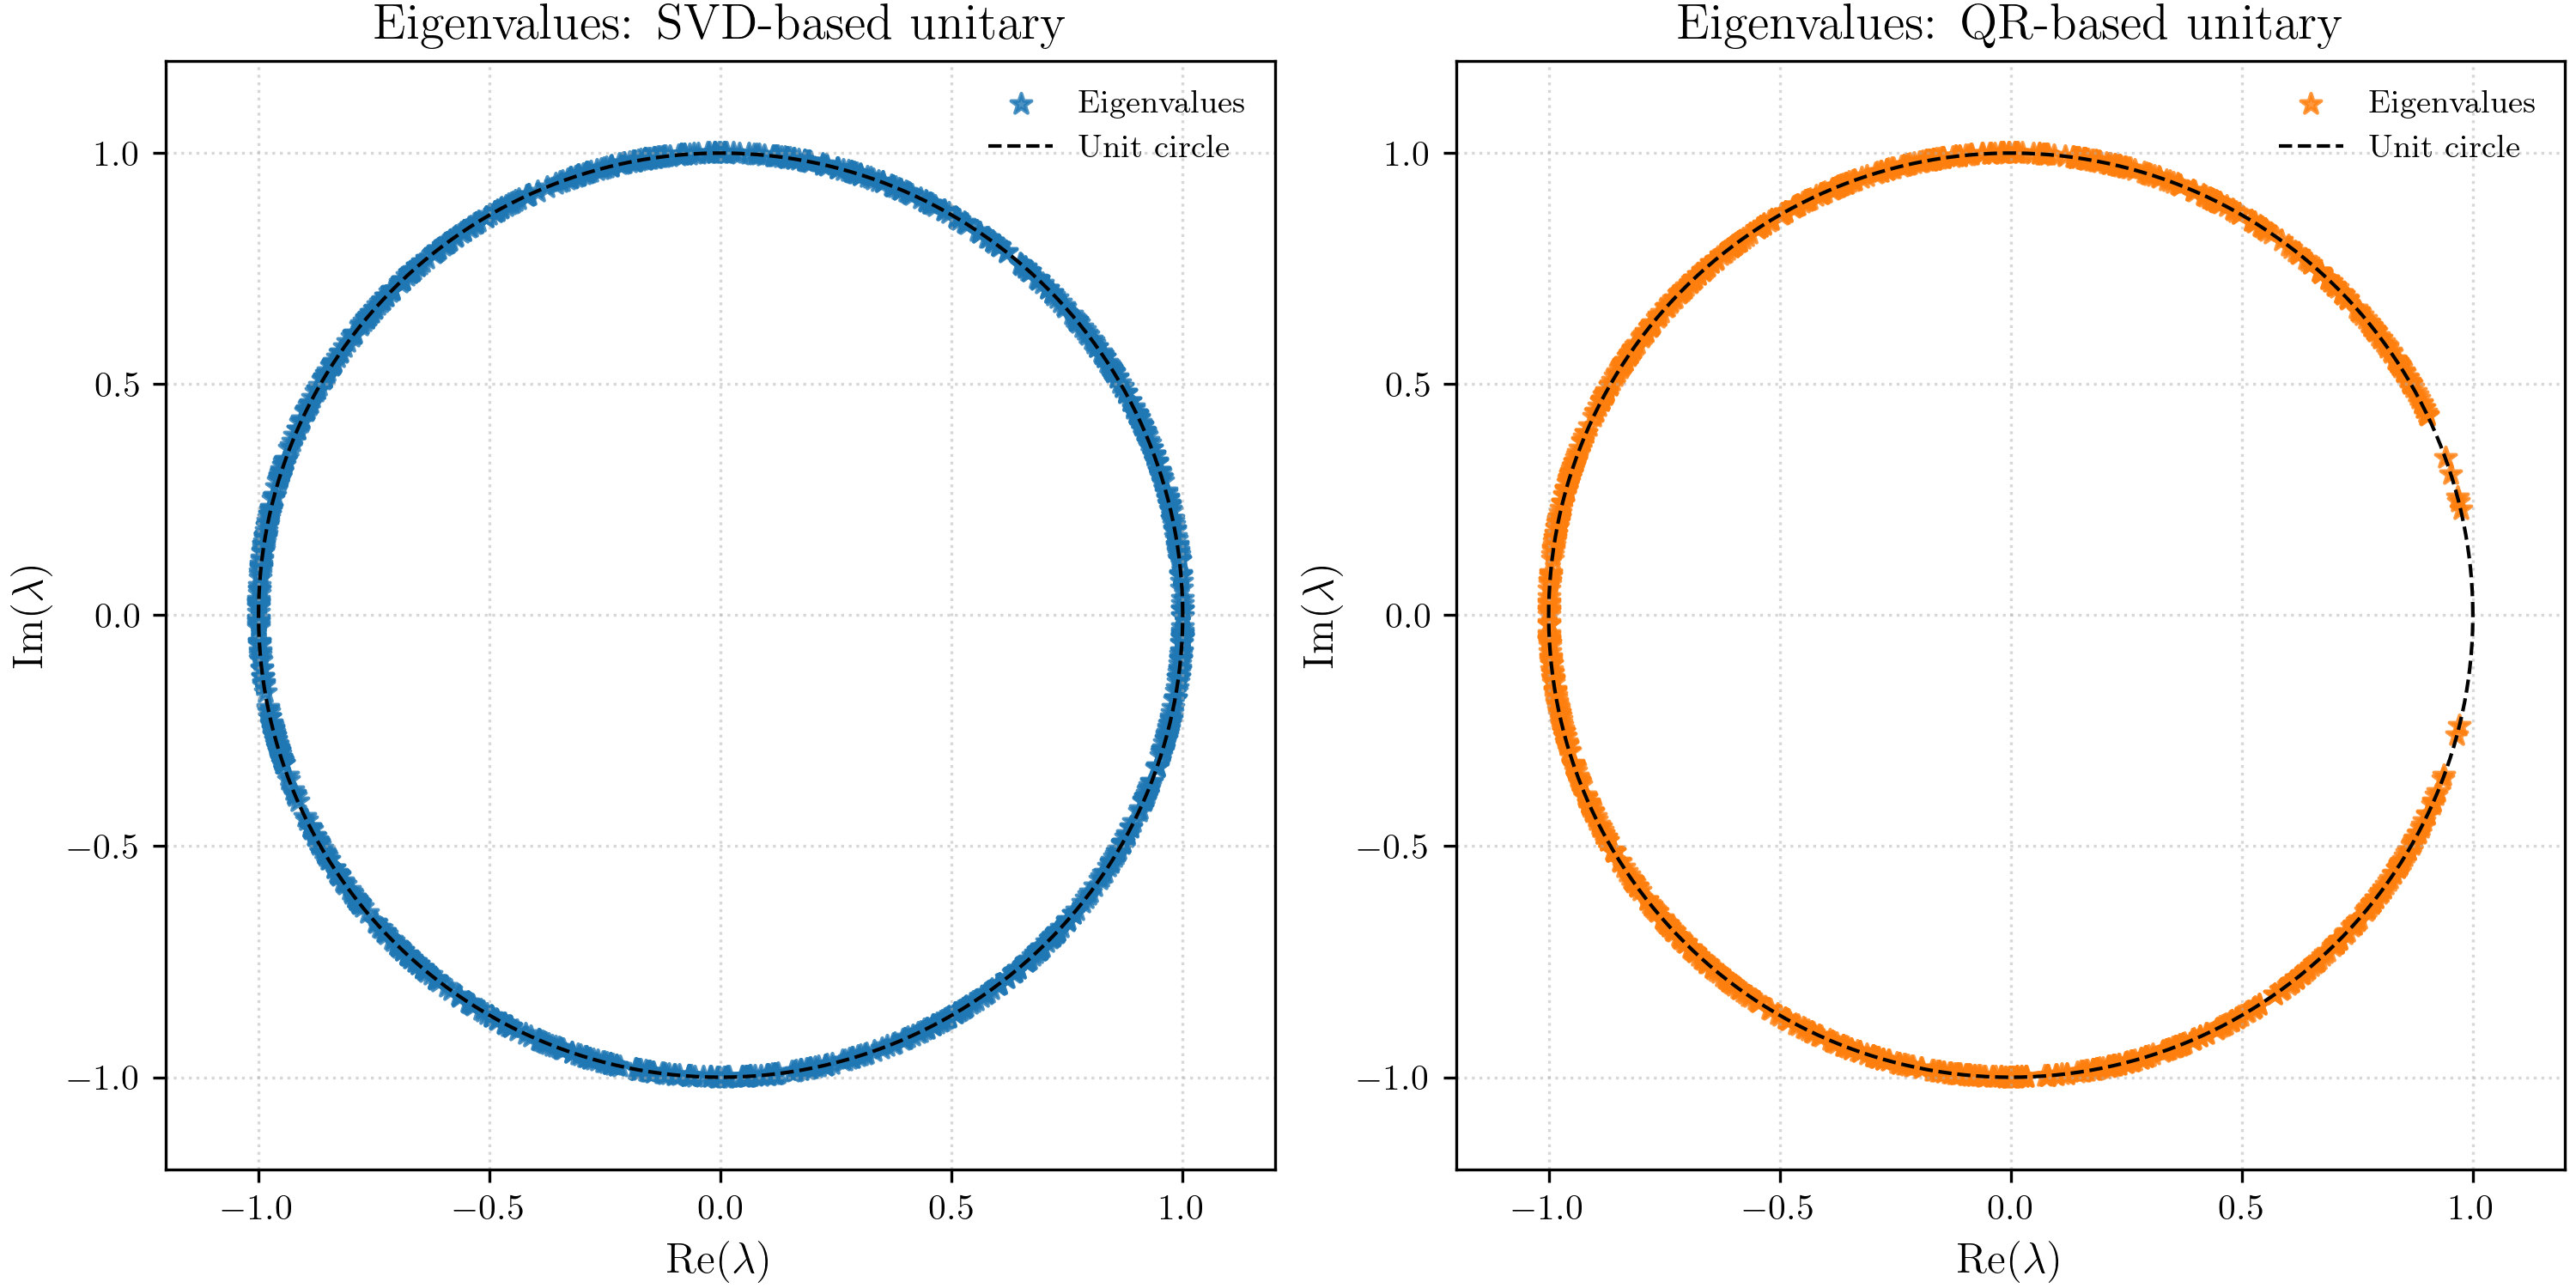
\includegraphics[width=1\textwidth]{Graphics/eigenvalue_comparison.png}
    \caption{Eigenvalue distributions of random unitary matrices generated via SVD and QR.}
    \label{fig:eigenvalue-comparison}
\end{figure}

We can now compare the spectral density of a SVD-based random unitary matrix $U$ with that of a QR-based random unitary matrix $Q$. We also show how the $\sigma$ influences the plots.

\begin{figure}[H]
    \centering
    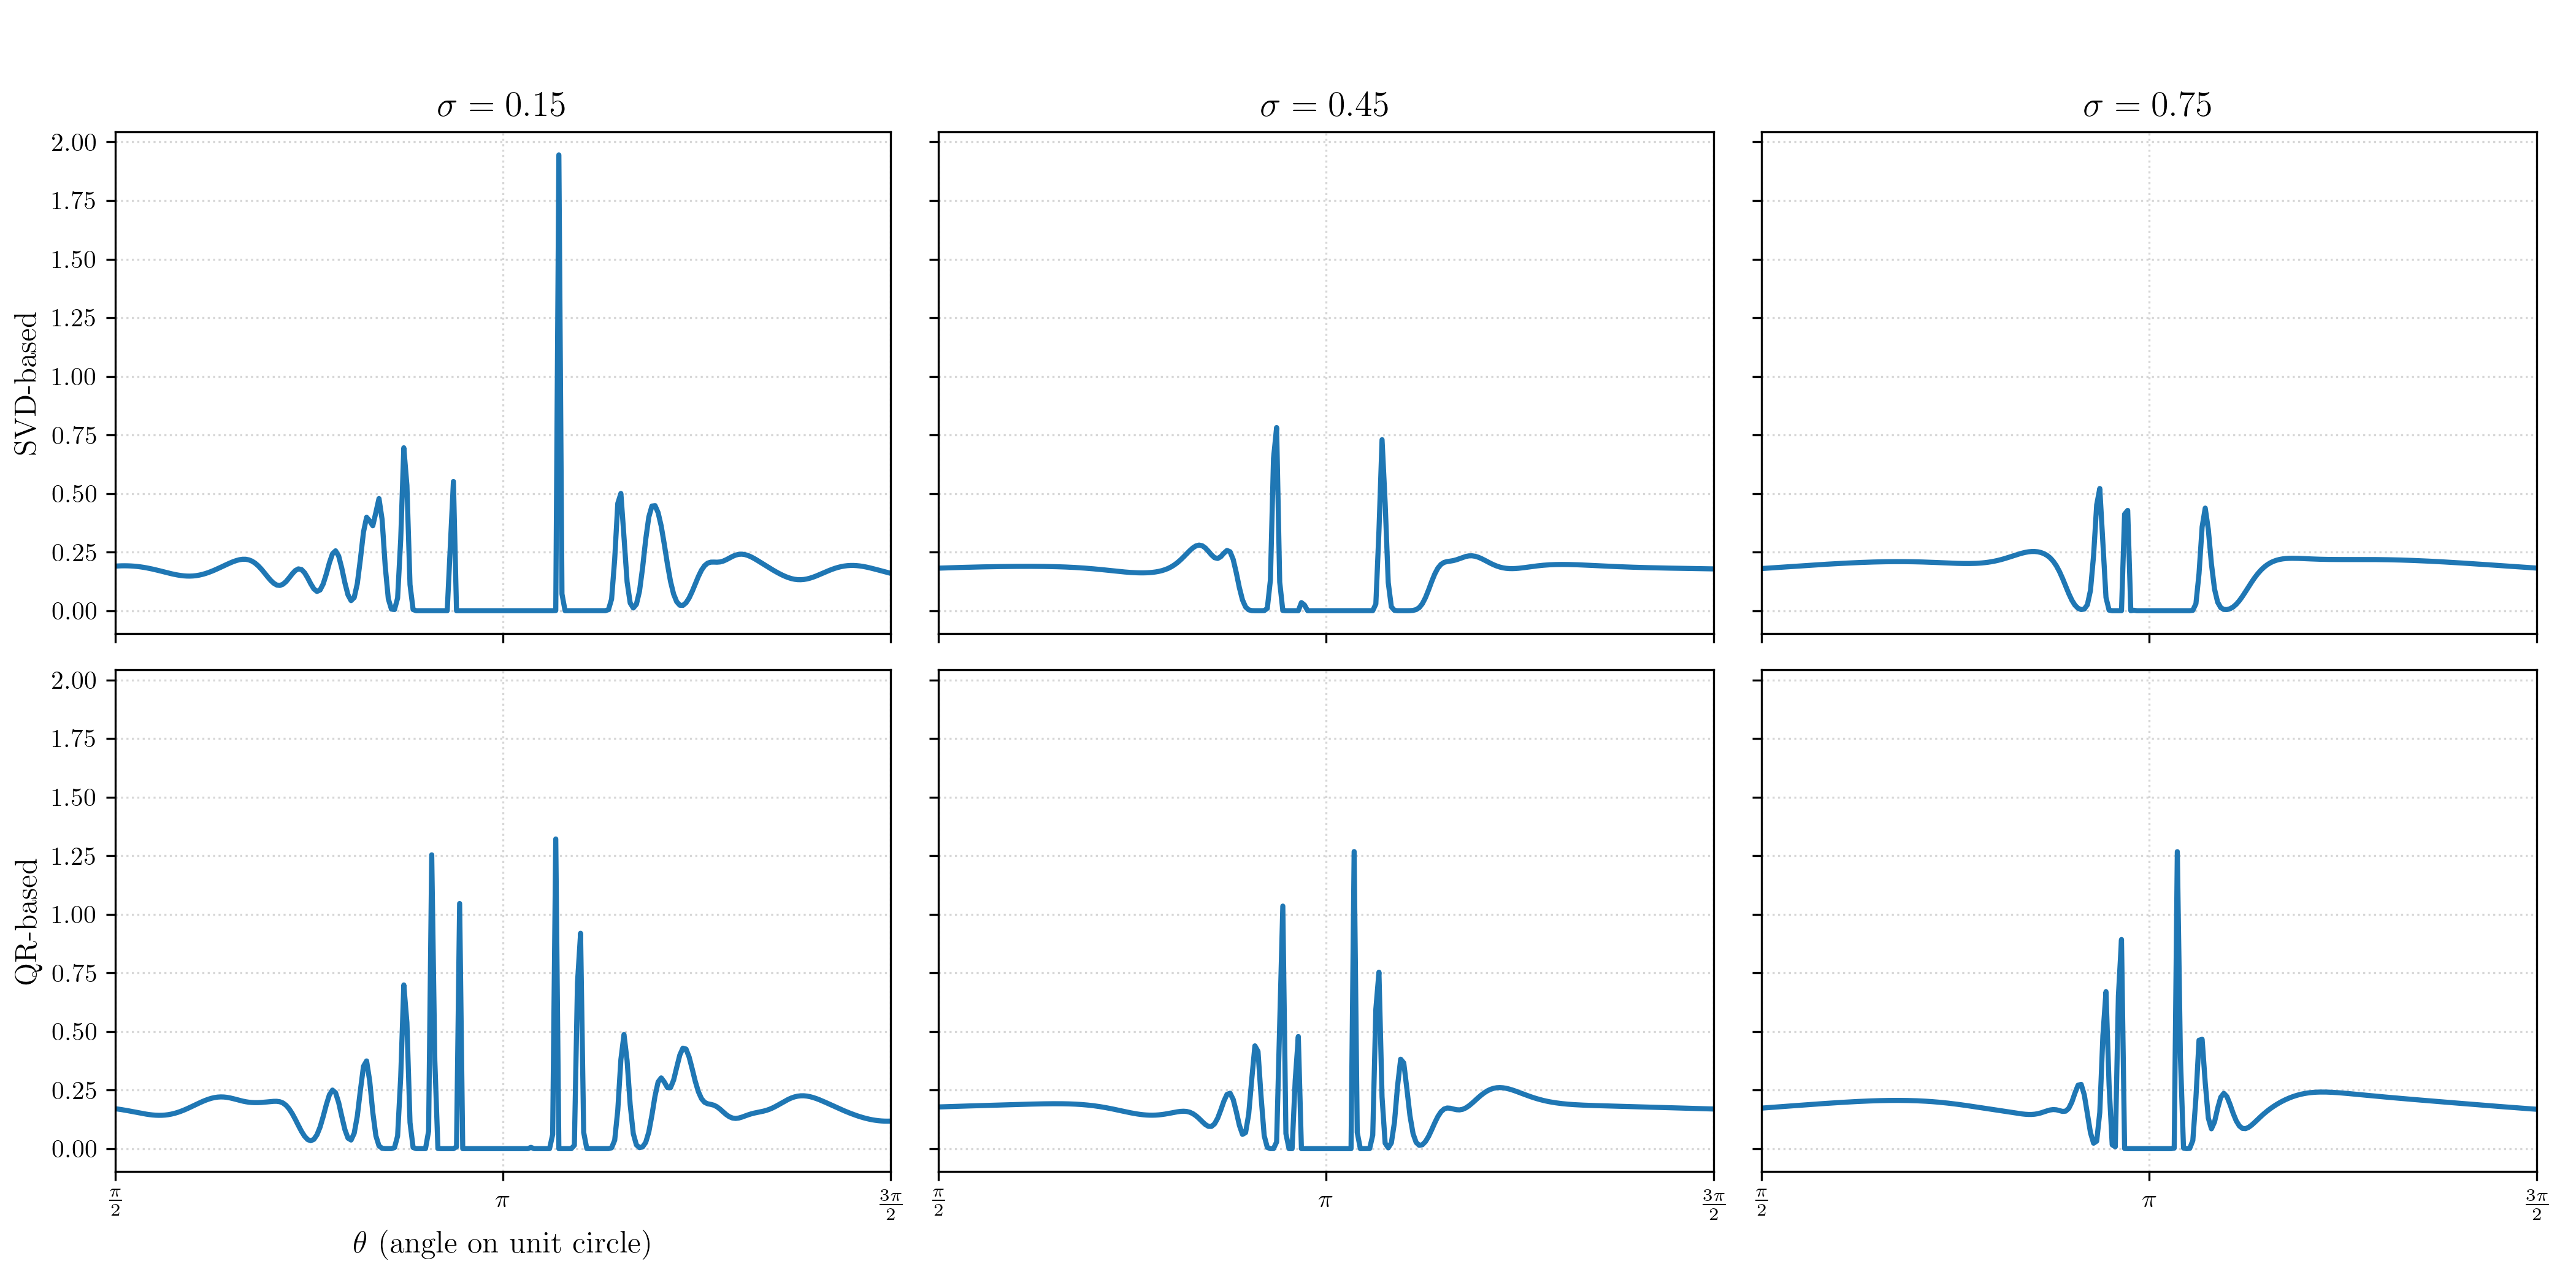
\includegraphics[width=1\textwidth]{Graphics/compare_svd_qr_spectral_density.png}
    \caption{Regularized spectral density of random unitary matrices generated via SVD and QR for varying $\sigma$.}
    \label{fig:spectral_density_comparison}
\end{figure}

It is evident, that a bigger $\sigma$ leads to a smoother spectral density but at the cost of losing information, while a smaller $\sigma$ captures more fine-grained features. This behavior is consistent across both SVD-based and QR-based random unitary matrices.

With this understanding of the spectral density and the choice of random unitary matrices, we can now proceed to implement the Kernel Polynomial Method (KPM) to compute the spectral density numerically. Below are the results of applying the KPM to both SVD-based and QR-based random unitary matrices.

\begin{figure}[H]
    \centering
    \begin{minipage}{0.49\textwidth}
        \centering
        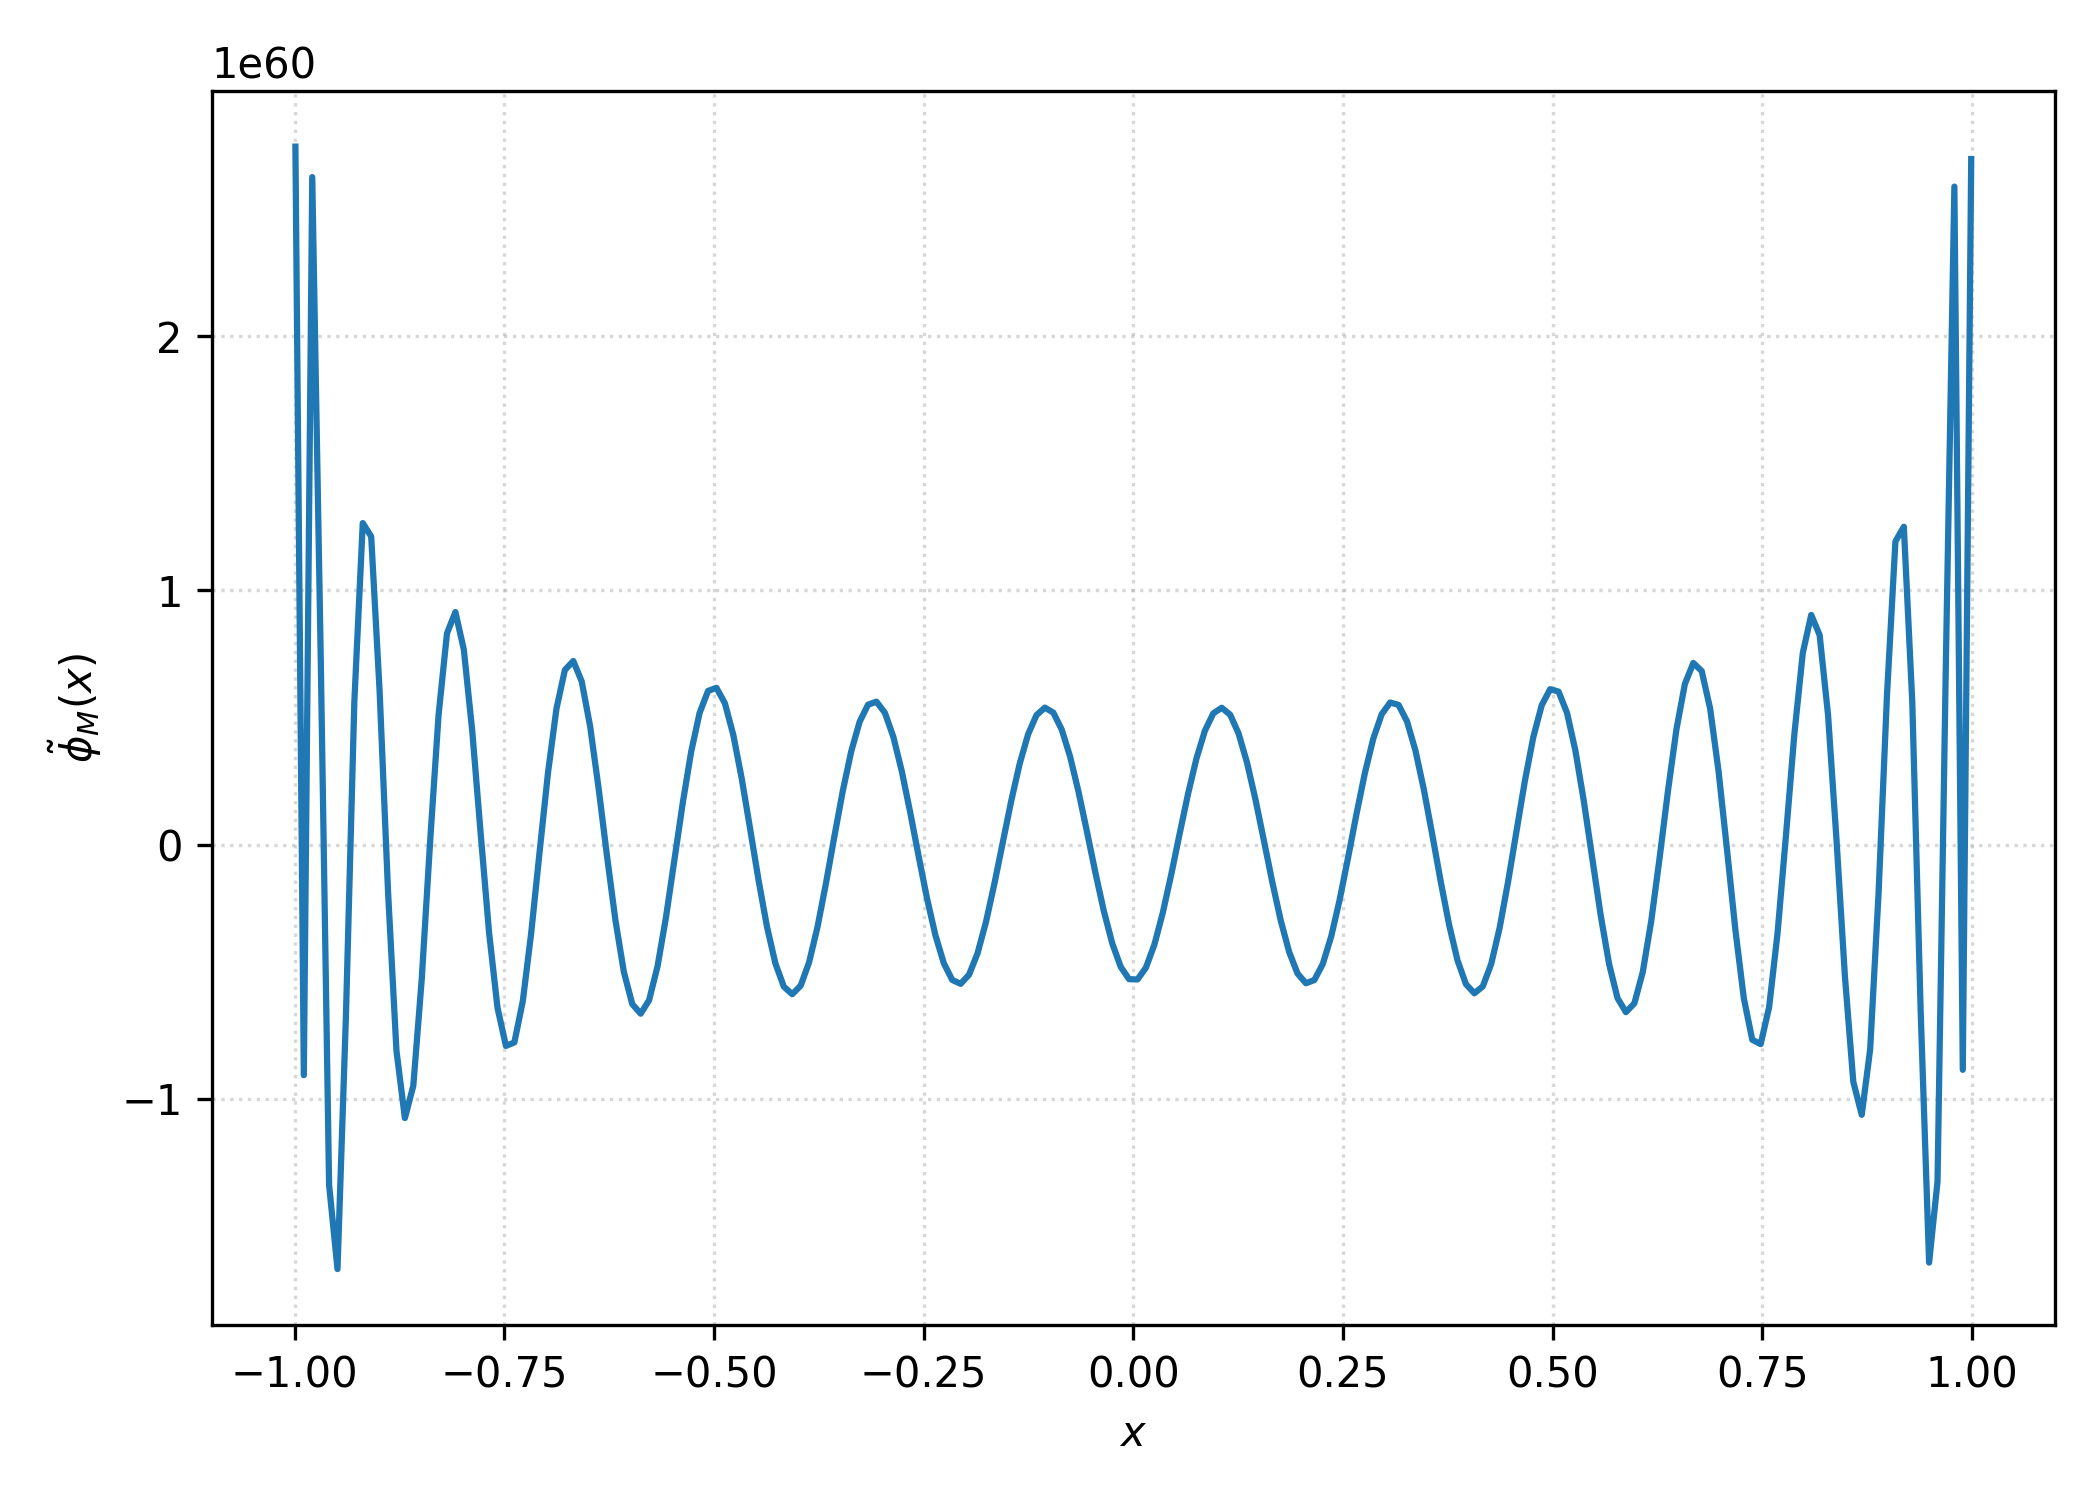
\includegraphics[width=\textwidth]{Graphics/svd_kpm.png}
        \subcaption{SVD-based}
    \end{minipage}
    \hfill
    \begin{minipage}{0.49\textwidth}
        \centering
        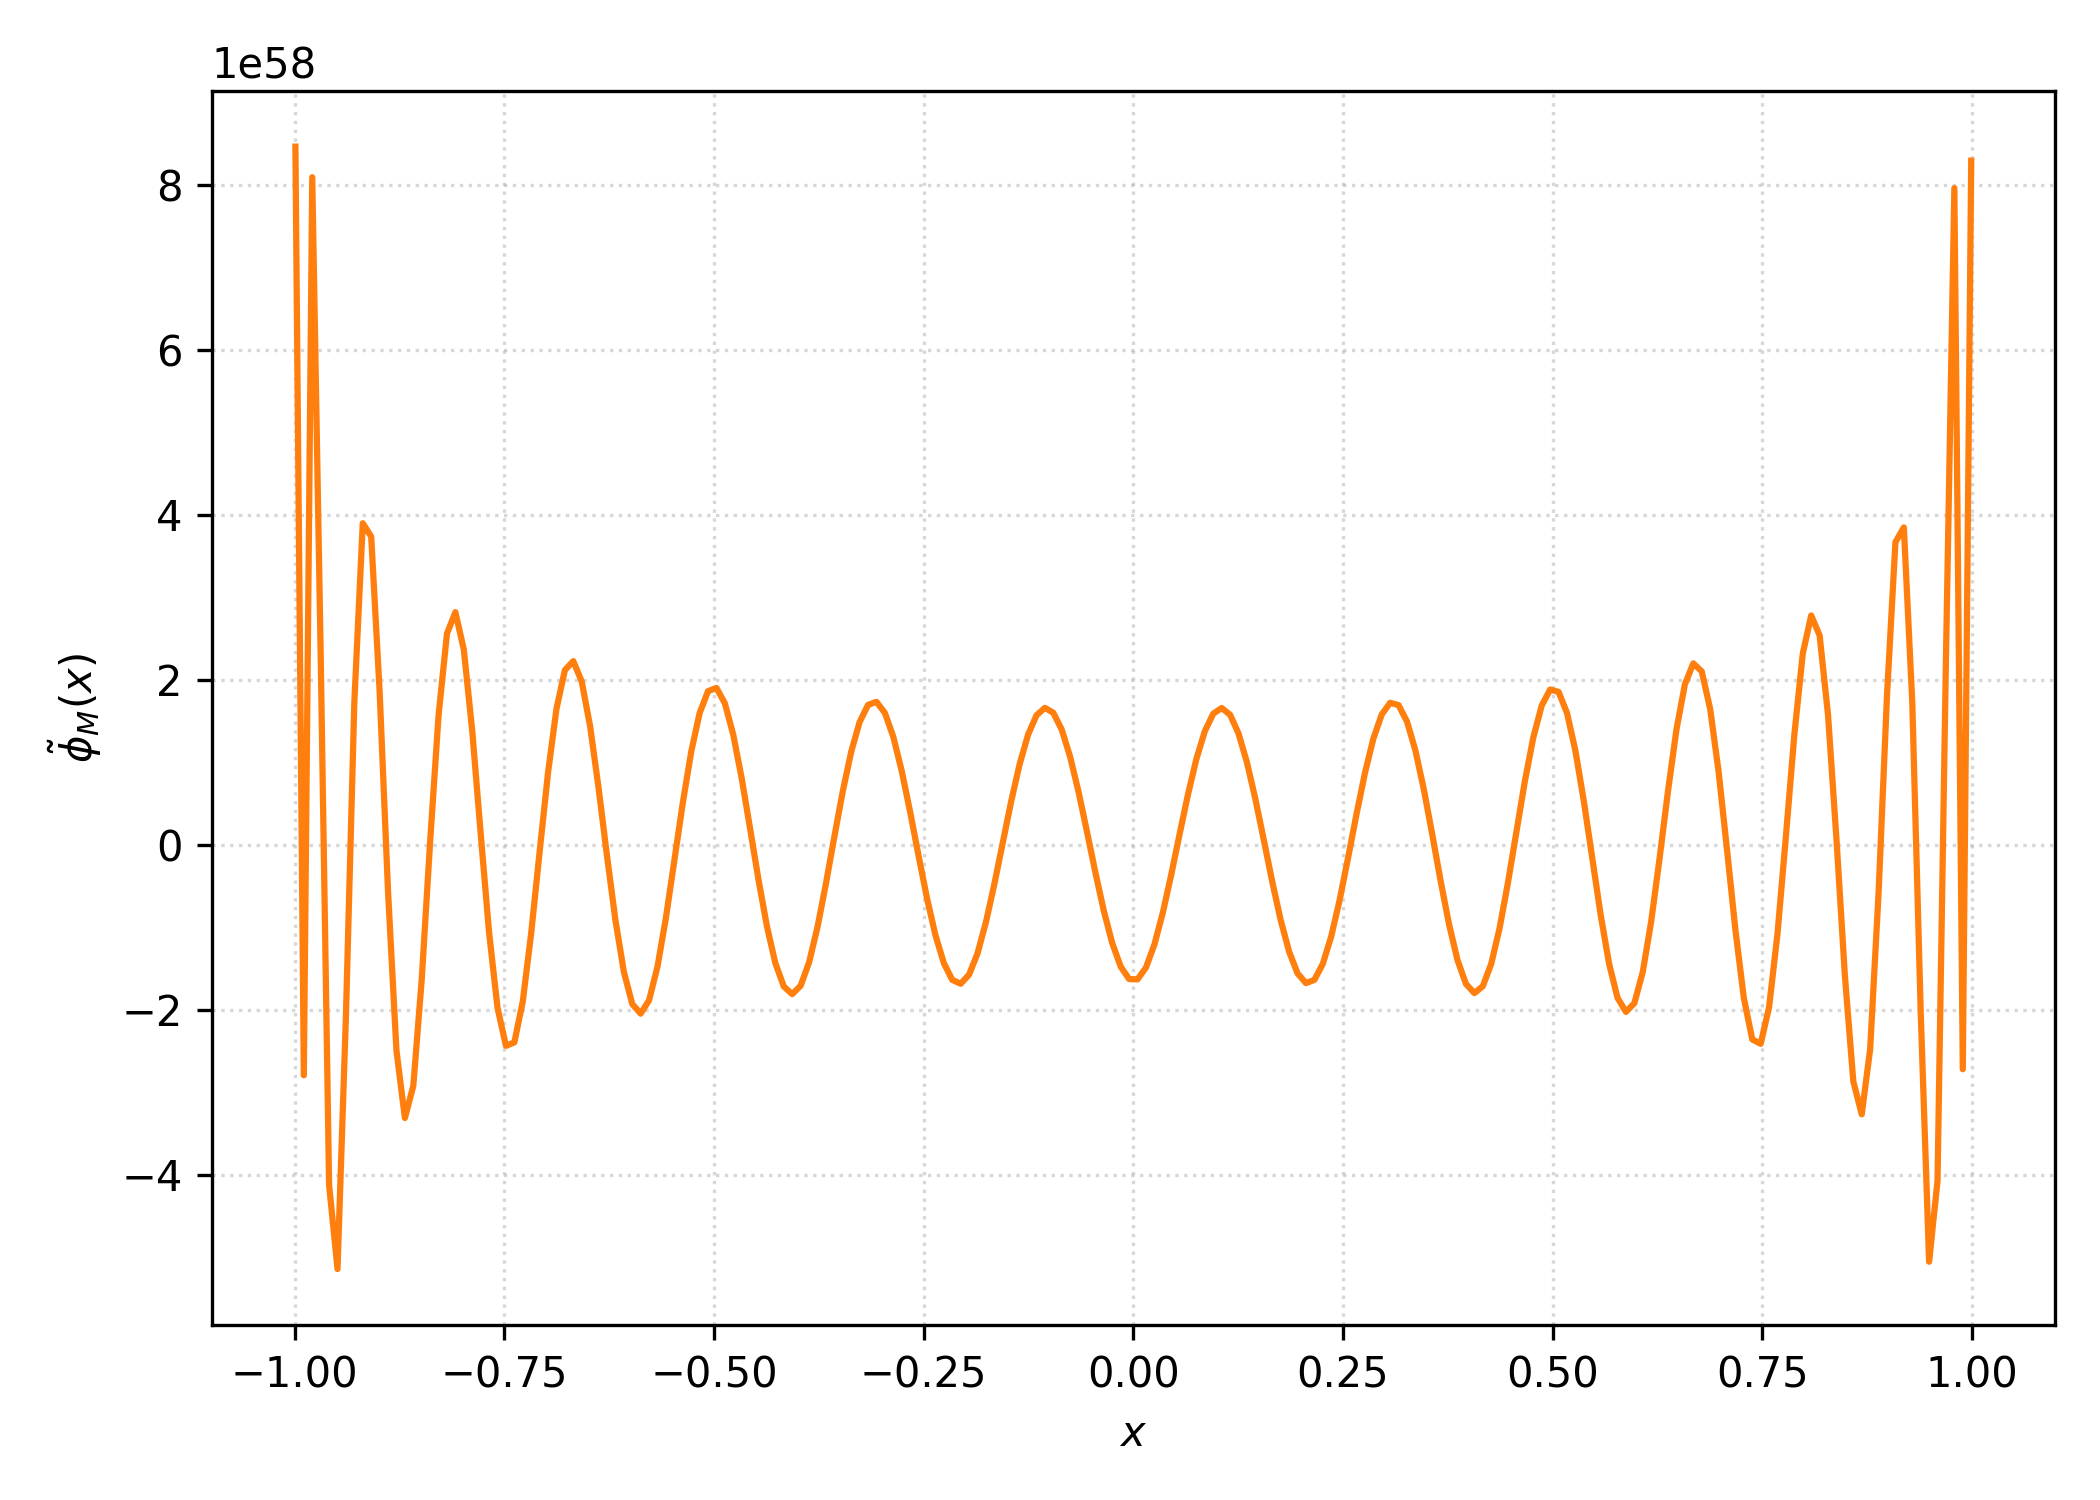
\includegraphics[width=\textwidth]{Graphics/qr_kpm.png}
        \subcaption{QR-based}
    \end{minipage}
    \caption{KPM spectral density estimates for random unitary matrices}
    \label{fig:compare_svd_qr_kpm}
\end{figure}

In comparison to the theoretical spectral density, the KPM estimates show large oscillations, so called \emph{Gibbs oscillations}, which are a common artifact of polynomial approximations. These oscillations can be mitigated by using a larger number of Chebyshev polynomials in the KPM, but this also increases the computational cost. It is also obvious that the KPM hurts the principle of non-negativity of the spectral density, as it can yield negative values in the estimates. This is a known limitation of the KPM and can be addressed by some sophisticated techniques in the future.

\chapter{Appendix}
\section{The Jacobian for the Cayley Transform}

To compute the Jacobian for the Cayley transform $\varphi: \R \to S^1$, let $x \in \mathbb{R}$. Then
\[
\varphi(x) = \frac{i - x}{i + x} = -\frac{x^2 - 1}{x^2 + 1} + i \frac{2x}{x^2 + 1}.
\]
The derivative of $\varphi$ and its inverse are computed as follows:
\[
\hat{\varphi} =
\begin{bmatrix}
    -\frac{x^2 - 1}{x^2 + 1}, & \frac{2}{x^2 + 1} \\
\end{bmatrix}
\implies \frac{\dphi}{\dx} =
\begin{bmatrix}
    -\frac{4x}{(x^2 + 1)^2}, & \frac{2 - 2x^2}{(x^2 + 1)^2} \\
\end{bmatrix}
\]
by the quotient rule. The norm of the derivative is then

\[
\left \| \frac{\dphi}{\dx} \right \| = \sqrt{\left(-\frac{4x}{(x^2 + 1)^2}\right)^2 + \left(\frac{2 - 2x^2}{(x^2 + 1)^2}\right)^2} = \sqrt{\frac{16x^2 + 4 - 8x^2 + 4x^4}{(x^2 + 1)^4}} = \frac{2}{x^2 + 1}.
\]

Therefore, the Jacobian for the transformation from $z$ to $w$ is
\[
J(z) = \left| \frac{dw}{dz} \right| = \frac{2}{(z^2 + 1)}
\]
and the inverse Jacobian is $\frac{z^2 + 1}{2}$.

Thus, to transform the spectral density from the real line to the unit circle, we multiply by
\[
\frac{x^2 + 1}{2}
\]
This factor accounts for the change of variables and ensures that the density is properly normalized on the unit circle. (See handwritten notes for the derivation.)

\section{Source Code and Materials}
Below is the link to our GitHub repository, which contains both the LaTeX source files for this thesis and the executable, self-written Python code implementing the Kernel Polynomial Method.

\noindent
\url{https://github.com/ClarinaSaxel/spectral-density-of-unitary-matrices}

\section{Declaration of Independent Work}
I hereby declare that I have written this thesis independently and have not used any sources or aids other than those indicated. All passages taken from other works, either verbatim or in substance, have been identified as such.

\section{Zusammenfassung (Deutsch)}
Diese Bachelorarbeit behandelt die numerische Approximation der Spektraldichte unitärer Matrizen mit der Kernel-Polynom-Methode (KPM). Es werden die mathematischen Grundlagen, die Regularisierung der Spektraldichte, die Anwendung der KPM sowie numerische Ergebnisse vorgestellt und diskutiert. Die Arbeit wurde in englischer Sprache verfasst; diese Zusammenfassung erfolgt gemäß den formalen Anforderungen in deutscher Sprache.

\bibliographystyle{plain}
\begin{thebibliography}{56}

    \bibitem{baer18}
    \textsc{C. Bär},
    \textit{Lineare Algebra und analytische Geometrie},
    Springer Spektrum
    2018.

    \bibitem{golub2013matrix}
    \textsc{G. H. Golub and C. F. Van Loan},
    \textit{Matrix Computations},
    4th edition,
    Johns Hopkins University Press,
    Baltimore, MD,
    2013.

    \bibitem{sheldonaxler}
    \textsc{S. Axler},
    \textit{Linear Algebra Done Right},
    Springer,
    2015.

    \bibitem{higham}
    \textsc{N. J. Higham},
    \textit{Functions of Matrices: Theory and Computation},
    SIAM,
    2008.

    \bibitem{strichartz}
    \textsc{R. S. Strichartz},
    \textit{A Guide to Distribution Theory and Fourier Transforms},
    World Scientific,
    2003.

    \bibitem{reichl}
    \textsc{L. E. Reichl},
    \textit{A Modern Course in Statistical Physics},
    4th edition,
    Wiley-VCH,
    2016.

    \bibitem{sakurainapolitano}
    \textsc{J. J. Sakurai and J. Napolitano},
    \textit{Modern Quantum Mechanics},
    2nd edition,
    Addison-Wesley,
    2011.

    \bibitem{oppenheimschafer}
    \textsc{A. V. Oppenheim and R. W. Schafer},
    \textit{Discrete-Time Signal Processing},
    3rd edition,
    Prentice Hall,
    2010.

    \bibitem{mitra}
    \textsc{S. K. Mitra},
    \textit{Digital Signal Processing: A Computer-Based Approach},
    2nd edition,
    McGraw-Hill Science Engineering Math,
    2001.

    \bibitem{nortonkarczub}
    \textsc{M. P. Norton, D. G. Karczub},
    \textit{Fundamentals of Noise and Vibration Analysis for Engineers},
    Cambridge University Press,
    2003.

    \bibitem{mezzadri2007}
    \textsc{F. Mezzadri},
    \textit{How to generate random matrices from the classical compact groups},
    Notices of the AMS, 54(5), 592--604, 2007.
    doi:10.1090/noti209

    \bibitem{andersonguionnetzeitouni}
    \textsc{G. W. Anderson, A. Guionnet, O. Zeitouni},
    \textit{An Introduction to Random Matrices},
    Cambridge University Press,
    2010.

    \bibitem{weisse2006}
    \textsc{A. Weisse, G. Wellein, A. Alvermann, H. Fehske},
    \textit{The kernel polynomial method},
    Reviews of Modern Physics, 78(1): 275--306, 2006.
    doi:10.1103/RevModPhys.78.275

    \bibitem{linsaadyang14}
    \textsc{L. Lin, Y. Saad, C. Yang},
    \textit{Approximating Spectral Densities of Large Matrices},
    SIAM Review, 58(1): 34--65, 2016.
    doi:10.1137/130933381

    \bibitem{richtmyer}
    \textsc{R. D. Richtmyer},
    \textit{Principles of Advanced Mathematical Physics},
    vol 1, Springer Verlag,
    New York,
    1981.

    \bibitem{PasSh11}
    \textsc{L. Pastur, M. Shcherbina},
    \textit{Eigenvalue Distribution of Large Random Matrices},
    AMS,
    2011.

\end{thebibliography}

\end{document}